\documentclass[conference]{IEEEtran}
\usepackage[T1]{fontenc}
\usepackage{amsmath,amssymb}
\usepackage{cite}
\usepackage{booktabs}
\usepackage{graphicx}
\usepackage{xurl}
\usepackage{hyperref}
\hypersetup{
  colorlinks=true,
  linkcolor=blue,
  urlcolor=blue,
  citecolor=blue,
  pdfauthor={Jabulani Monchwe, Martin Chanza, Olorato Motitswane, Mfundo Monchwe}
}
\newcommand{\software}{\textsf{ReliableML}}
\newcommand{\code}[1]{\texttt{\small #1}}
\newcommand{\jabulaniauthor}{
\IEEEauthorblockN{Jabulani Monchwe}
\IEEEauthorblockA{\textit{Applied Business Analytics and Decision Making}\\
\textit{North-West University}\\
\textit{IDEA-Research Club Chairperson}\\
Johannesburg, South Africa\\
\href{mailto:monchwej.25@gmail.com}{monchwej.25@gmail.com}}
}
\newcommand{\martinchanzauthor}{
\IEEEauthorblockN{Martin Chanza}
\IEEEauthorblockA{\textit{Applied Business Analytics and Decision Making}\\
\textit{North-West University}\\
Mafikeng, South Africa\\
\href{mailto:martin.chanza@nwu.ac.za}{martin.chanza@nwu.ac.za}}
}
\newcommand{\oloratoauthor}{
\IEEEauthorblockN{Olorato Motitswane}
\IEEEauthorblockA{\textit{Eduvos Midrand Campus -- IT Faculty Data Science, South Africa}\\
\textit{IDEA-Research Club}\\
\href{mailto:oloratomotitswane@gmail.com}{oloratomotitswane@gmail.com}}
}
\newcommand{\mfundoauthor}{
\IEEEauthorblockN{Mfundo Monchwe}
\IEEEauthorblockA{\textit{Eduvos Midrand Campus -- IT Faculty Data Science, South Africa}\\
\textit{IDEA-Research Club}\\
\href{mailto:diditmfundo@gmail.com}{diditmfundo@gmail.com}}
}
\newcommand{\minenhleauthor}{
\IEEEauthorblockN{Minenhle Mchunu}
\IEEEauthorblockA{\textit{Applied Business Analytics and Decision Making}\\
\textit{Eduvos Midrand Campus -- IT Faculty Data Science, South Africa}\\
\textit{IDEA-Research Club}\\
\href{mailto:Mchunu.minenhle02@gmail.com}{Mchunu.minenhle02@gmail.com}}
}
\newcommand{\projecturl}{\url{https://github.com/Jabualani/ML-Reliabilty}}

\title{Data Intelligence and Visualization for Reliable Machine Learning: Target and Feature Diagnostics, and Pure-NumPy Outlier Detection with Isolation Forest, LOF and Self-Organising Maps}
\author{\jabulaniauthor
\and
\martinchanzauthor
\and
\oloratoauthor
\and
\mfundoauthor}
\hypersetup{pdfauthor={Jabulani Monchwe, Martin Chanza, Olorato Motitswane, and Mfundo Monchwe}}
\begin{document}
\maketitle
\begin{abstract}
Most reliability failures of a deployed model are decided before any model is fitted: a leaking column, a target that the features cannot explain, a pair of columns measuring the same quantity, or a handful of records that do not belong to the population. \software{} \code{DataIntelligence} is a single module that investigates a table before modelling. It answers what happened (profiles, hazards, tails), why (association, partial correlation, driver chains, sub-populations) and what then (trend, stationarity, autocorrelation), and it audits the target (leakage, label-permutation explainability, alternative targets) and the features (hazard filters, correlation and VIF pruning, multi-method ranking). This paper gives the exact mathematics of every statistic, and details the outlier layer: a robust Mahalanobis distance, an isolation forest, the local outlier factor and a batch self-organising map, all implemented in NumPy, combined into a vote-based consensus and displayed in figures designed to surface unusual records and structure. On planted-outlier benchmarks no single detector wins every scenario: LOF is near perfect for local-density outliers (AUROC 0.999) where the global detectors are near chance, while the isolation forest is the only method above chance for outliers lying between clusters (AUROC 0.947). The equal-weight ensemble is therefore a triage tool, not a replacement for reading the individual detectors. A toolkit adds power analysis (predictive, explanatory and statistical), hypothesis tests and A/B testing, root-cause search, time-series analysis, iterative distribution-aware feature construction with an untouched holdout, and active-learning row selection with a plug-in hook for external selectors, each with measured results. Nothing is written to disk unless the user asks for it.
\end{abstract}
\begin{IEEEkeywords}
exploratory data analysis, data leakage, multicollinearity, isolation forest, local outlier factor, self-organising map, visualization, reliability
\end{IEEEkeywords}
\section{Introduction}
Reliability of a learned model is bounded by the reliability of its data. A leaking feature inflates validation scores and then collapses in production; collinear features make coefficients unstable and attributions arbitrary; a target that is mostly noise cannot be rescued by a better learner; and a small group of anomalous records can dominate a fit or, conversely, be the most valuable cases in the table. \software{} already monitors a fitted model (distribution shift, deterioration, fairness, explanation consistency). \code{DataIntelligence} moves the same discipline upstream, to the data.

The module lives in one file, \code{src/ml\_reliability/data\_intelligence.py}, and is organised around three questions: what happened, why it happened, and what happens next. It adds two layers that are specific to supervised learning, \emph{target intelligence} and \emph{feature intelligence}, and a figure layer that turns each finding into a picture. The design follows four rules.
\begin{enumerate}
\item \textbf{Own models.} Every model used inside the engine (KNN, ridge and logistic regression, k-means, the isolation forest, LOF and the self-organising map) comes from StatCore or from NumPy in this module; scikit-learn is not imported. \code{scipy.stats} and \code{statsmodels} are used for classical statistics and \code{matplotlib}/\code{seaborn} for figures.
\item \textbf{Association is not causation.} Causal language is limited to \emph{screening}: partial correlations are reported as associational evidence.
\item \textbf{The target is never read where it must not be.} In \code{scope="multicollinearity"} the engine only sees $X$, so it is safe inside an AutoML training partition.
\item \textbf{Nothing is saved by default.} Figures and reports are written only when the user passes \code{plot\_dir} or \code{export\_dir}, or calls \code{export}; \code{plot()} returns in-memory figures.
\end{enumerate}
Section~\ref{sec:arch} describes the architecture, Sections~\ref{sec:profile}--\ref{sec:target} the statistics, Section~\ref{sec:outliers} the outlier layer, Section~\ref{sec:viz} the visualizations, and Section~\ref{sec:exp} measured results and their limits.

\section{Architecture and modes}\label{sec:arch}
\code{DataIntelligence(mode, \ldots).analyze(df, target\_column, time\_column, user\_question)} returns a \code{DataIntelligenceReport} holding a summary score $S\in[0,100]$ and a details dictionary. The mode selects the stages: \code{comprehensive\_eda}, \code{target\_intelligence}, \code{feature\_intelligence}, \code{field\_investigation}, \code{auto\_question\_generator}, \code{llm\_augmented} and \code{autonomous} (all stages). Stages are listed in Table~\ref{tab:stages}.
\begin{table}[t]\caption{Stages of the engine and the question each answers.}\label{tab:stages}\centering\scriptsize
\begin{tabular}{@{}p{1.2cm}p{2.2cm}p{4.3cm}@{}}\toprule
Pillar & Stage & Question \\\midrule
What happened & profile, hazards, tails & Are the columns usable? Constant, quasi-constant, high-cardinality, skewed, missing? \\
Why & association, drivers, clusters, outlier ensemble, SOM & What moves with what? Which sub-populations and unusual records exist? \\
What then & trend, ADF, autocorrelation & Is there drift in time that breaks i.i.d. validation? \\
Target & leakage, explainability, alternatives & Can the target be learned honestly, and is it the best target? \\
Features & VIF, correlation pruning, ranking & Which columns are redundant, which carry signal? \\\bottomrule
\end{tabular}\end{table}
An optional LLM backend (a callable, \code{ollama} or a custom URL) receives only a statistical summary, never raw rows, and only when configured.

\subsection{Summary score}
Let $\bar m$ be the mean missing percentage, $h$ the number of hazard columns, $q$ the number of strongly related pairs and $f$ the multivariate-outlier fraction. The data score is
\begin{equation}\label{eq:score}S_{\text{data}}=100-\min(15,\bar m)-\min(15,3h)-\min(10,2q)-\min(10,100f),\end{equation}
clipped to $[0,100]$, and $S$ is the mean of $S_{\text{data}}$ and the target and feature scores when those stages ran. The score is a triage signal for ordering datasets, not a calibrated probability.

\section{What happened: profiling}\label{sec:profile}
For a numeric column $x_1,\ldots,x_n$ the engine reports the mean $\bar x$, standard deviation $s$, quantiles at $\{1,5,25,50,75,95,99\}\%$, skewness and excess kurtosis
\begin{equation}g_1=\frac{\tfrac1n\sum_i(x_i-\bar x)^3}{\left(\tfrac1n\sum_i(x_i-\bar x)^2\right)^{3/2}},\quad g_2=\frac{\tfrac1n\sum_i(x_i-\bar x)^4}{\left(\tfrac1n\sum_i(x_i-\bar x)^2\right)^{2}}-3.\end{equation}
Normality is assessed with the Shapiro--Wilk statistic and the Kolmogorov--Smirnov distance $D=\sup_t|F_n(t)-\Phi((t-\bar x)/s)|$ to the fitted normal. The Tukey fences $[Q_1-1.5\,\mathrm{IQR},\,Q_3+1.5\,\mathrm{IQR}]$ give the univariate tail counts. Hazards are constant columns ($s=0$), quasi-constant columns (one level with share $\ge0.99$) and high-cardinality categorical columns; identifier-like columns are handled by the leakage screen (Section~\ref{sec:target}). A column is skew-flagged when $|g_1|>2$.

\section{Why: association, drivers and sub-populations}\label{sec:assoc}
\subsection{Pairwise association}
For numeric pairs the engine reports Pearson $r$, Spearman $\rho$ (Pearson on ranks) and Kendall $\tau$ (on a seeded sample of at most $1500$ rows). Dependence beyond monotone trends is measured by mutual information on quantile-binned columns,
\begin{equation}I(A;B)=\sum_{a,b}p(a,b)\ln\frac{p(a,b)}{p(a)p(b)},\end{equation}
with ten quantile bins. Categorical--categorical association uses Cram\'er's $V=\sqrt{\chi^2/(n(\min(r,c)-1))}$, and numeric--categorical association uses the correlation ratio $\eta=\sqrt{SS_{\text{between}}/SS_{\text{total}}}$. A pair is \emph{strong} when $|r|\ge0.7$ or $|\rho|\ge0.7$.

\subsection{Drivers and chains}
For a numeric target field $y$ the drivers are the features ranked by $\max(|r|,|\rho|)$, each with a Pearson $p$-value. A multi-hop chain lists, for each of the top three drivers $d$, the other columns $c$ with $|r(d,c)|\ge0.5$: these are candidates for mediating or confounding relations and are \emph{not} causal claims. When there is no numeric target, the field of interest is the column with the largest coefficient of variation.

\subsection{Partial correlation}
Given a feature $x_j$, the target $y$ and the remaining features $Z$, the partial correlation is
\begin{equation}r_{x_jy\cdot Z}=\frac{-P_{jy}}{\sqrt{P_{jj}P_{yy}}},\end{equation}
where $P=(R+10^{-6}I)^{-1}$ is the regularised inverse of the correlation matrix $R$ of the numeric features and $y$. With marginal $r=r_{x_jy}$ and partial $r'=r_{x_jy\cdot Z}$, the report flags (a) a sign flip ($rr'<0$ with both $|r|,|r'|>0.1$, suppression), (b) $|r|>0.3$ and $|r'|<0.3|r|$ (the association is carried by other features: a shared cause or proxy), and (c) $|r'|>1.5|r|$ with $|r'|>0.2$ (a suppressor effect). These are cautions for coefficient interpretation, not causal conclusions.

\subsection{Sub-populations}
Standardised numeric columns are clustered with StatCore k-means with silhouette-selected $k\in[2,6]$. For a row $i$ with in-cluster mean distance $a(i)$ and nearest other-cluster mean distance $b(i)$, the silhouette is $s(i)=(b(i)-a(i))/\max(a(i),b(i))$ \cite{rousseeuw1987}. Each cluster is summarised by the three columns whose cluster mean differs most from the grand mean, in standard deviations.

\section{Multicollinearity, VIF and feature pruning}\label{sec:vif}
With $R$ the correlation matrix of the numeric columns, the variance inflation factor of column $j$ equals
\begin{equation}\mathrm{VIF}_j=\frac1{1-R_j^2}=[R^{-1}]_{jj},\end{equation}
where $R_j^2$ is the coefficient of determination of $x_j$ regressed on all other columns \cite{belsley1980}. The engine adds $10^{-9}I$ before inversion and clips VIFs to $[1,10^6]$. The condition number of the correlation matrix is $\kappa=\sqrt{\lambda_{\max}/\lambda_{\min}}$, with a warning at $\kappa>30$.

\textbf{Redundant groups.} Pairs whose association (absolute Pearson for numeric pairs, Cram\'er's $V$ or $\eta$ for mixed pairs) reaches the threshold (default $0.90$) are reported, and union--find merges them into redundant clusters. \textbf{Pruning.} While $\max_j\mathrm{VIF}_j>\tau$ (default $\tau=10$) the engine drops the column with the largest VIF; among columns within $5\%$ of the maximum, the one with the lowest priority is dropped first. With no target (the multicollinearity scope) the priority is constant, so ties fall to the larger VIF. In AutoML the hook runs this on the training partition only and never reads the label, so it cannot leak into cross-validation.

\section{Target and feature intelligence}\label{sec:target}
\subsection{Leakage screen}
A feature is flagged when (i) its single-feature cross-validated skill reaches the leakage threshold (default $0.95$), (ii) its association with the target reaches that threshold (suspected duplicate or derived target), (iii) for regression $|\rho|\ge0.999$ (monotone copy), (iv) it is identifier-like (integer-like or categorical with at least $95\%$ unique values; medium severity), (v) its name contains the target name or looks like an after-the-fact field (outcome, result, future, \ldots) while being predictive (single-feature skill $>0.3$), or (vi) for categorical columns, missingness itself predicts the target (skill $\ge0.2$). Single-feature skill is cross-validated: classification uses balanced accuracy rescaled by chance, $\text{skill}=(\mathrm{BA}-1/K)/(1-1/K)$; regression uses $R^2$. The screen is a necessary hygiene check, not a proof: a legitimate but perfectly predictive input will also be flagged and should be reviewed by a domain expert.

\subsection{Explainability by label permutation}
Let $\hat s$ be the best cross-validated skill among a ridge/logistic model and a KNN model, and $\hat s^{(1)},\ldots,\hat s^{(B)}$ the skills obtained after permuting the labels ($B=20$ by default). The one-sided p-value is
\begin{equation}p=\frac{1+\#\{b:\hat s^{(b)}\ge\hat s\}}{1+B}.\end{equation}
With $B=20$ the smallest attainable $p$ is $1/21\approx0.048$, so the engine additionally records whether $\hat s$ exceeds \emph{every} permutation skill, and a target is declared noise only when it neither beats the null maximum nor has $p\le0.05$, or when $\hat s<0.02$. Verdicts are ``not distinguishable from noise'', ``weakly explained'' ($\hat s<0.15$) and ``strongly explained''. A learning curve at $75\%$ and $100\%$ of the rows is recorded to show whether more data would help.

\subsection{Alternative targets and feature search}
The engine builds alternative targets and evaluates each with the same cross-validated linear and KNN skill against the same $X$. For regression these are $\log(y-\min y+1)$, $\sqrt{y-\min y}$, a rank-Gauss transform $\sqrt2\,\mathrm{erf}^{-1}(2r_i-1)$ with $r_i=(\mathrm{rank}_i-\tfrac12)/n$, the residual of $y$ after a linear fit on one of the four most associated numeric columns, the ratio $y/x_c$ (positive columns), and $2$--$4$ quantile classes. Targets built from a column remove that column from $X$ to avoid trivial leakage. For classification they are one-vs-rest views of up to five classes and progressively merged classes, merging at each step the pair the model confuses most. A transform is recommended only when it improves skill by more than $0.03$ over the original.

The feature search is a two-stage grid. Stage one pre-filters the pool ($\le30$ strongest columns) with \emph{none}, \emph{variance}, \emph{correlation pruning} or \emph{VIF pruning}; stage two selects with \emph{none}, \emph{association top-half}, \emph{mutual-information top-half}, \emph{lasso}, \emph{forward}, \emph{backward} or \emph{permutation} selection. Each of the $4\times7$ combinations is scored by cross-validated skill; identical subsets are merged and the best few, plus the full pool, are re-scored. In this full scope the pruning priority is the target association, so of two redundant columns the one that is more related to the target is kept. \code{FeatureIntelligence} adds a separate multi-method ranking (mutual information, ANOVA $F$, $\chi^2$, recursive elimination, model importance) aggregated by rank percentile. These experiments are \emph{exploratory}: choosing the best among many candidates on the same data is a selection step, so its optimism must be re-estimated on untouched data. A known limitation is that a leaking column, if not excluded first, will win the selection (observed in our own demonstration, Fig.~\ref{fig:dash}); act on the leakage screen before adopting a subset.

\section{Outlier and structure detection}\label{sec:outliers}
Let $Z\in\mathbb R^{n\times p}$ be the numeric block, with missing values filled by the column median. All detectors run on one seeded sample of at most $n_{\max}=2000$ rows (\code{outlier\_max\_rows}), because LOF needs $O(n^2)$ memory.

\subsection{Robust Mahalanobis distance}
With coordinate-wise median $m$ and scaled median absolute deviation $\mathrm{MAD}_j=1.4826\,\mathrm{median}_i|z_{ij}-m_j|$, set $u_i=(z_i-m)/\mathrm{MAD}$ and
\begin{equation}d_i^2=u_i^\top\hat\Sigma_u^{-1}u_i,\qquad \hat\Sigma_u=\mathrm{Cov}(u)+10^{-6}I.\end{equation}
Under approximate normality $d_i^2\sim\chi^2_p$, so a row is flagged when $d_i^2>\chi^2_{p}(0.999)$. The location and scale are robust, but the covariance is the ordinary sample covariance of the scaled data, so a cluster of outliers can inflate it and mask itself (the ``masking'' effect, visible in Section~\ref{sec:exp}). Cost is $O(np^2+p^3)$.

\subsection{Isolation forest}
Following Liu et al.\ \cite{liu2008}, a tree is grown on a subsample of size $\psi=\min(256,n)$ by repeatedly choosing a feature $q$ uniformly among those with positive range in the node, and a split value uniformly in $[\min,\max]$ of that feature, until the node is a singleton or the height limit $\lceil\log_2\psi\rceil$ is reached. The path length of a row $x$ is
\begin{equation}h(x)=e(x)+c(\mathrm{size}(x)),\end{equation}
where $e(x)$ is the number of edges to the external node and $c$ corrects for unbuilt subtrees,
\begin{equation}c(m)=\begin{cases}2\,(\ln(m-1)+\gamma)-\dfrac{2(m-1)}{m},&m>2,\\1,&m=2,\\0,&m\le1,\end{cases}\end{equation}
with $\gamma\approx0.5772$ Euler's constant. The anomaly score averages over $T=100$ trees,
\begin{equation}s(x)=2^{-\mathbb E[h(x)]/c(\psi)}\in(0,1),\end{equation}
so values near $1$ are isolated quickly (anomalous) and values near $0.5$ or below are typical. The engine flags rows whose robust $z$-score $(s-\mathrm{median}(s))/(1.4826\,\mathrm{MAD}(s))$ exceeds $3.5$, instead of a fixed $0.5$ threshold, because the score scale depends on the data. Cost is $O(T\psi\log\psi+Tn\log\psi)$ and the model never forms an $n\times n$ matrix.

\subsection{Local outlier factor}
Following Breunig et al.\ \cite{breunig2000}, let $d_k(a)$ be the distance from $a$ to its $k$-th nearest neighbour, $N_k(a)$ its $k$ nearest neighbours (exactly $k$ points; ties broken arbitrarily), and
\begin{align}
\mathrm{rd}_k(a,b)&=\max\{d_k(b),d(a,b)\},\\
\mathrm{lrd}_k(a)&=\Big(\tfrac1k\textstyle\sum_{b\in N_k(a)}\mathrm{rd}_k(a,b)\Big)^{-1},\\
\mathrm{LOF}_k(a)&=\frac1k\sum_{b\in N_k(a)}\frac{\mathrm{lrd}_k(b)}{\mathrm{lrd}_k(a)}.
\end{align}
Inliers have $\mathrm{LOF}\approx1$; the engine flags $\mathrm{LOF}>1.5$ with $k=20$ on standardised columns. Because the score is a \emph{ratio} of local densities, a point can be flagged next to a dense cluster even when it is close to the bulk of the data, which global detectors cannot do. Cost is $O(n^2p)$ time and $O(n^2)$ memory.

\subsection{Self-organising map}
A self-organising map \cite{kohonen1982,kohonen2001} places $U=R\times C$ units on a rectangular grid with coordinates $r_u$ and weight vectors $w_u\in\mathbb R^p$. The best-matching unit of $x$ is $b(x)=\arg\min_u\|x-w_u\|$. The engine uses the batch algorithm: in epoch $t$ of $T=40$,
\begin{equation}w_u\leftarrow\frac{\sum_ih_{u,b(x_i)}(t)\,x_i}{\sum_ih_{u,b(x_i)}(t)},\quad h_{uv}(t)=\exp\!\Big(-\frac{\|r_u-r_v\|^2}{2\sigma_t^2}\Big),\end{equation}
with a neighbourhood radius that shrinks geometrically from $\sigma_0=\max(R,C)/2$ to $\sigma_T=0.7$ cells. Weights are initialised deterministically on the plane spanned by the first two principal components, $w_{(a,b)}=\bar x+t_a\sigma_1v_1+t_b\sigma_2v_2$ with $t$ evenly spaced in $[-2,2]$, so results do not depend on a random initial state. The grid is square with side $\mathrm{clip}(\lceil\sqrt{5\sqrt n}\,\rceil,4,12)$, i.e.\ about $5\sqrt n$ units. The map yields four diagnostics.
\begin{itemize}
\item \textbf{Quantization error} $\mathrm{QE}=\tfrac1n\sum_i\|x_i-w_{b(x_i)}\|$, per row and per unit (units with no hits are shown blank).
\item \textbf{Topographic error} $\mathrm{TE}=\tfrac1n\sum_i\mathbf 1[\text{best and second-best units are not grid neighbours}]$, with $8$-neighbourhood adjacency; high TE means the grid is folded and the picture misleading.
\item \textbf{U-matrix}: the mean weight-space distance from a unit to its four grid neighbours; ridges mark cluster borders and valleys mark clusters.
\item \textbf{Hit map} and \textbf{component planes}: counts per unit, and the value of one standardised feature across the grid. Planes for the three features with greatest variance across units are drawn.
\end{itemize}
A row is flagged by the SOM when the robust $z$-score of its quantization error exceeds $3.5$: it is far from \emph{every} prototype. Cost is $O(TnUp)$.

\subsection{Consensus}
Let $\phi_m(i)\in\{0,1\}$ be the flag of detector $m\in\{\text{IF},\text{LOF},\text{Maha},\text{SOM}\}$. The vote count is $v_i=\sum_m\phi_m(i)$ and the \emph{consensus} outliers are $\{i:v_i\ge2\}$. A rank score $\rho_i=\tfrac14\sum_m\mathrm{rank}_m(i)/n$ orders rows, and the ten rows with the highest $\rho_i$ are reported with the detectors that flagged them and the three standardised columns that drive the deviation. The report also lists, per detector, the rows flagged by that detector \emph{alone} (\code{single\_detector\_only}), because a single vote is exactly where a specialised detector sees something the others cannot (Section~\ref{sec:exp}).

\section{Question discovery: data without a question}\label{sec:questions}
A frequent starting point is a table and no question. \code{analyze} then returns a \emph{question plan}: a list of items, each with a category, a priority (high, medium, low), the question, the evidence that triggered it and the call that answers it. Priority is assigned by rule: target, structure and outlier items are high; relationship, category and missingness items are medium; distribution items are low.

\paragraph{Candidate targets.} Without a target, the engine ranks columns by how well the remaining numeric columns predict them. For a column $c$ (the eight numeric columns with the largest coefficient of variation and up to four categorical columns with at most ten levels), a ridge model is fitted on the other numeric columns with 3-fold cross-validation, and the out-of-fold skill is computed as in Section~\ref{sec:target}: $R^2$ for numeric $c$, chance-adjusted balanced accuracy for categorical $c$. Columns with $|r|\ge0.98$ to $c$ are removed from the predictors and reported as \code{derived\_from}, so a unit conversion cannot pass for a finding. The skill bands are: $\ge0.6$ strongly, $\ge0.3$ moderately, $\ge0.1$ weakly explained, otherwise not explainable. A high skill says that $c$ is \emph{learnable}, not that it is \emph{worth predicting}; the plan says so by asking the user to decide, and the next step is a full target-intelligence run on the chosen column.

\paragraph{Other generators.} Clusters with silhouette $\ge0.25$ produce a question about the smallest group and its signature; the outlier consensus produces a question naming the columns that drive the flagged rows; groups of three or more columns with $|r|>0.7$ ask whether they measure one latent quantity; a categorical level with share above $0.8$ asks whether rare levels are under-sampled; a categorical/numeric pair with $\eta\ge0.3$ asks whether the group effect is real or an artefact of measurement; for a column missing more than $5\%$, the missingness indicator is correlated with the numeric columns, and $|r|\ge0.3$ upgrades the item to high priority because the gaps are then informative; strong skew, a time column and exact duplicate rows each produce one item. All thresholds are heuristics chosen to keep the list short; they do not replace domain knowledge, and the items are prompts for investigation, not findings.

\section{Visualization for hidden gems}\label{sec:viz}
Every stage has a figure; figures use one house style (seaborn whitegrid, colour-blind palette, constrained layout) shared with the drift plots of \software{}. Table~\ref{tab:figs} states the question each figure is built to answer.
\begin{table*}[t]\caption{Figures produced by \code{DataIntelligence.plot()} and the question each answers.}\label{tab:figs}\centering\scriptsize
\begin{tabular}{@{}p{2.6cm}p{5.2cm}p{8.2cm}@{}}\toprule
Figure & Encoding & What to look for \\\midrule
\code{dashboard} & six panels: score, leakage bars, explainability, VIF, selection, correlation & one-page triage of the whole table \\
\code{distributions} & histogram+KDE, dashed ECDF on a second axis, mean line & skew, multimodality (a bump that the mean hides), clipping \\
\code{association} & bars of target association and single-feature skill, line at the leakage threshold & columns that predict the target too well to be honest \\
\code{correlation}, \code{feature\_ranking} & Pearson heatmap; rank-percentile heatmap by selection method & groups of columns moving together; features that every method ranks high \\
\code{vif} & horizontal bars on a log axis, line at $\tau$ & which columns to prune; log scale keeps $10$ and $500$ both readable \\
\code{explainability} & histogram of permuted-label skills, vertical lines for real skill & distance between the null and the real skill \\
\code{feature\_selection} & skill against subset size, all-features baseline & smallest subset that matches the baseline \\
\code{clusters}, \code{target\_candidates} & PCA plane coloured by k-means cluster; skill of each alternative target & sub-populations and their size; whether a transformed or merged target is more learnable \\
\code{outlier\_consensus} & PCA plane coloured by isolation score, consensus rows ringed; detector agreement; vote histogram (symlog) & which rows are unusual, by whom, and how many methods agree \\
\code{som} & U-matrix, hit map, per-unit quantization error, component planes & cluster borders, empty regions of feature space, regions where the data is poorly represented, and which features organise the map \\
\code{tails}, \code{missingness}, \code{trend} & standardised boxplots, missingness matrix, series with fitted trend & tail weight, structured missingness, drift in time \\\bottomrule
\end{tabular}\end{table*}
\begin{figure*}[t]\centering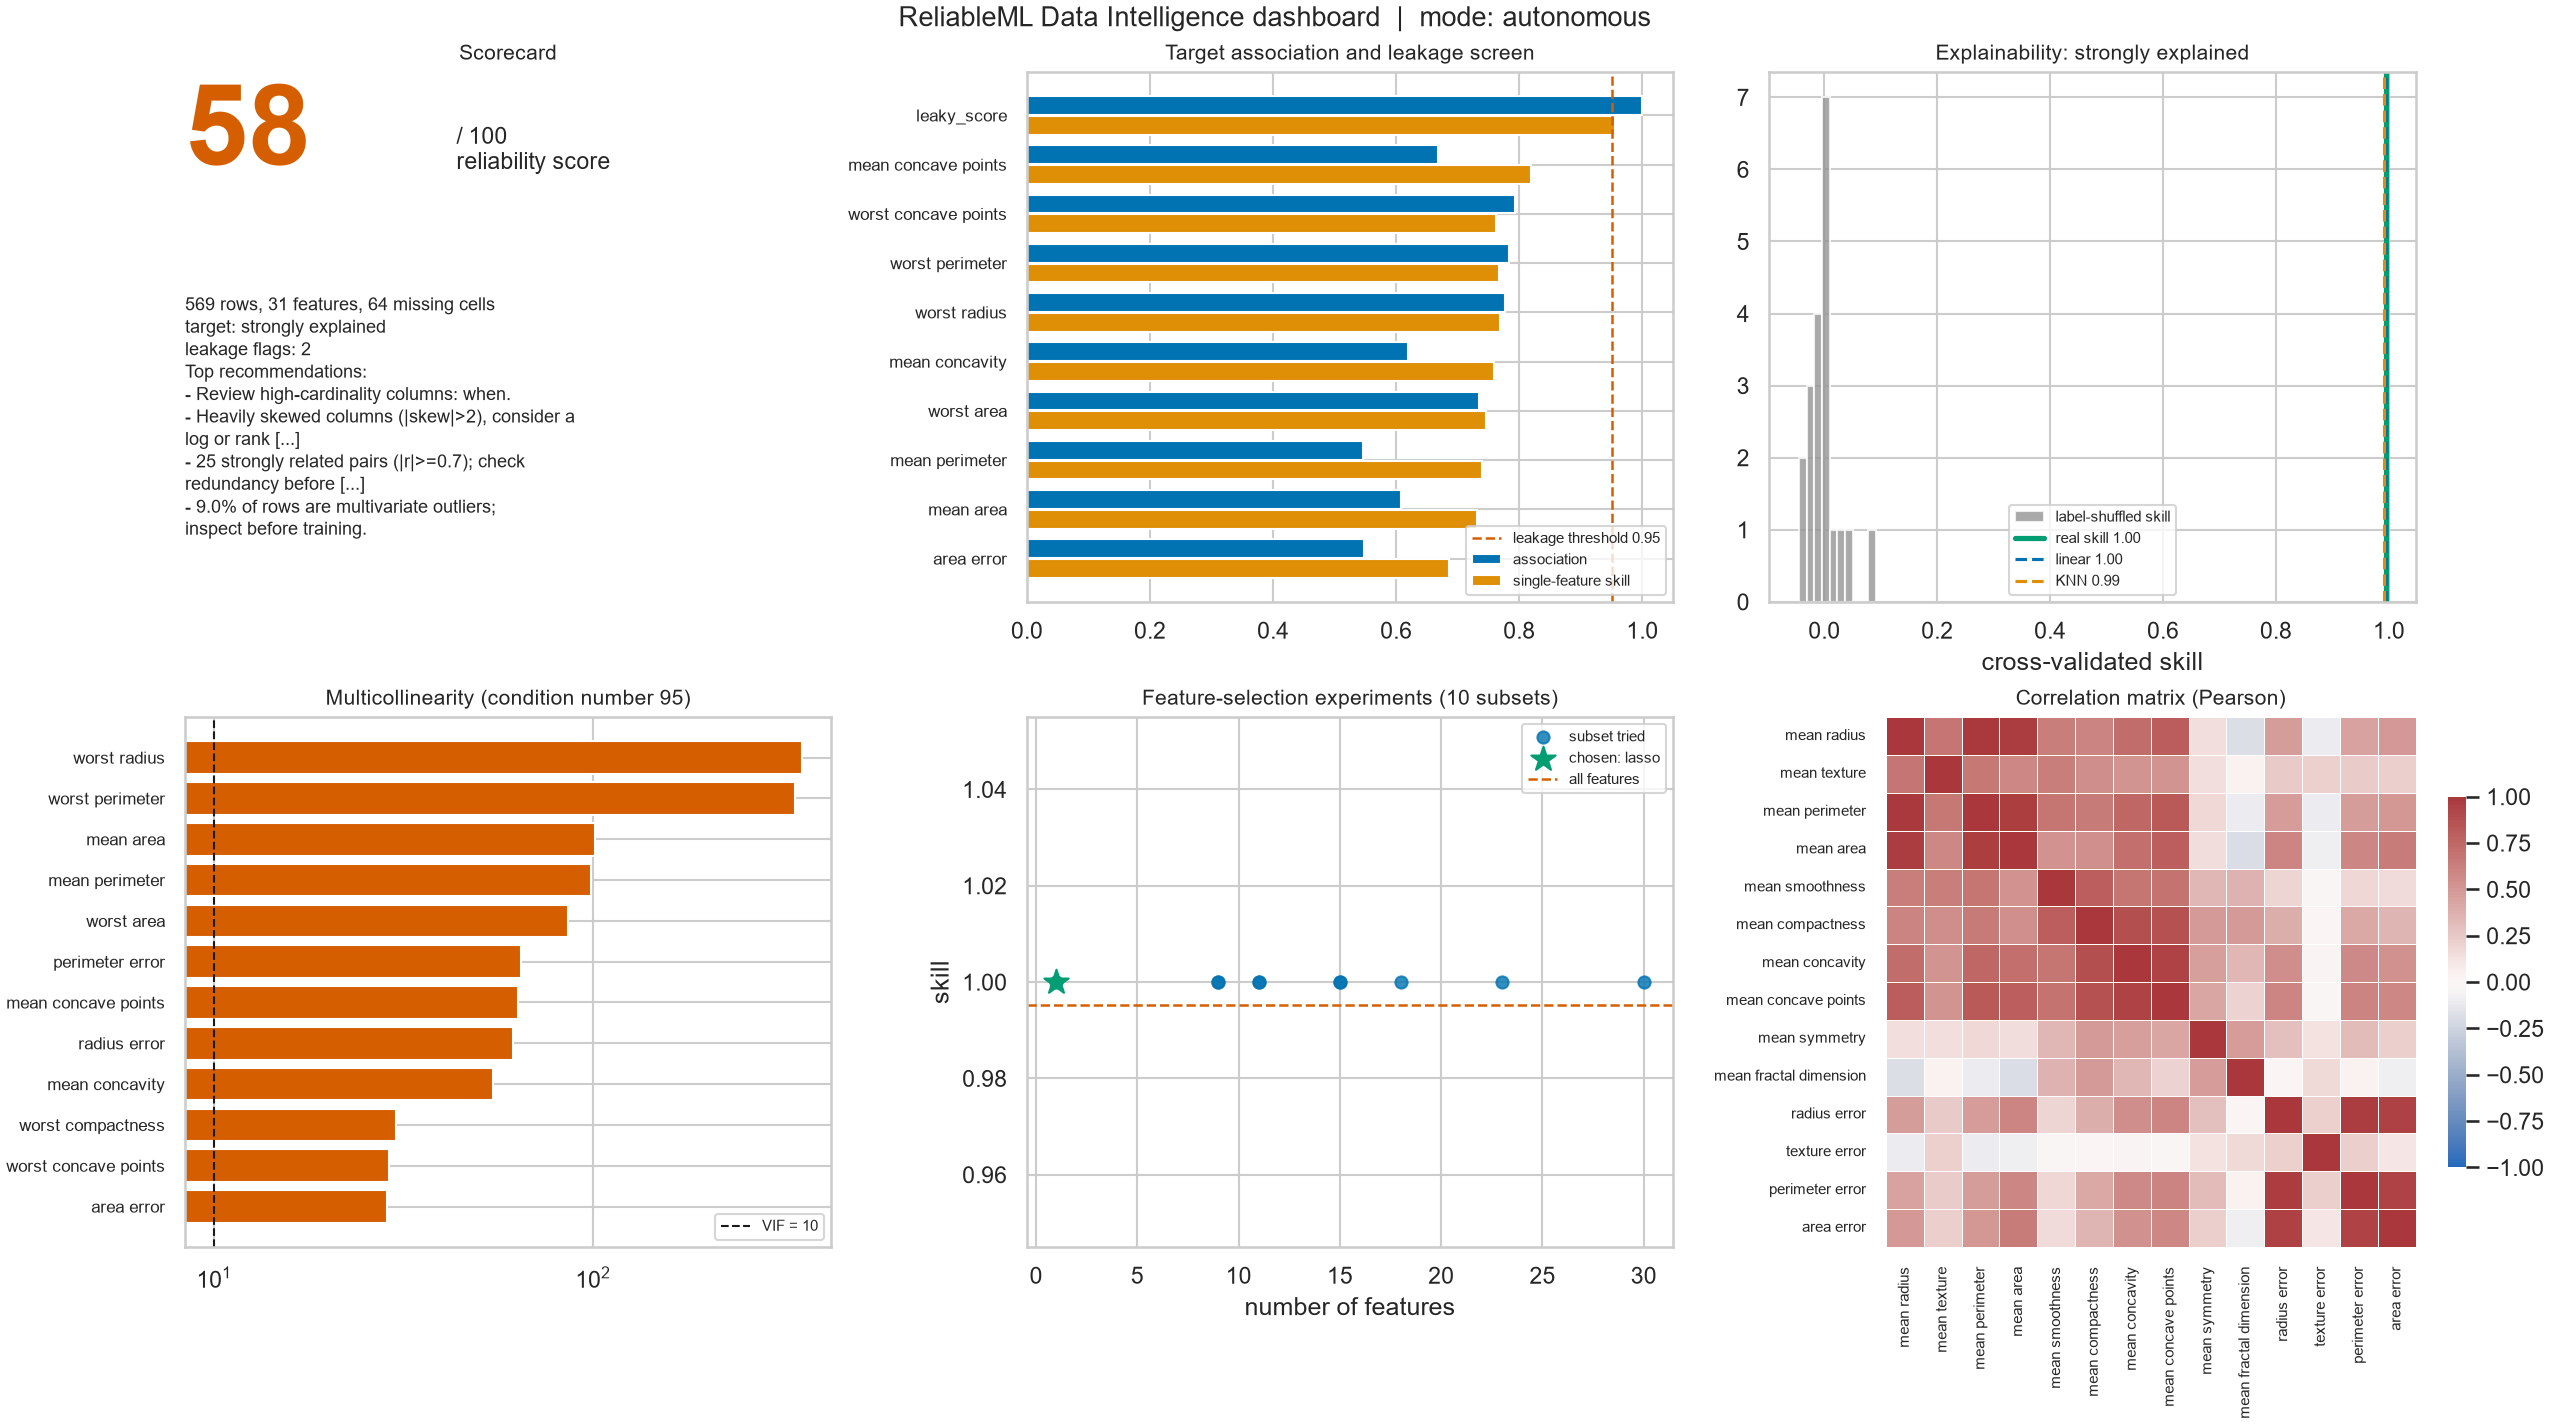
\includegraphics[width=\textwidth]{figures/dashboard.png}\caption{The dashboard for Breast Cancer with a planted leaking column (\code{leaky\_score}), planted outliers and missing values: the leakage bar crosses the $0.95$ threshold, the explainability panel separates the real skill from the permutation null, and the VIF panel shows the size-related block.}\label{fig:dash}\end{figure*}
\begin{figure*}[t]\centering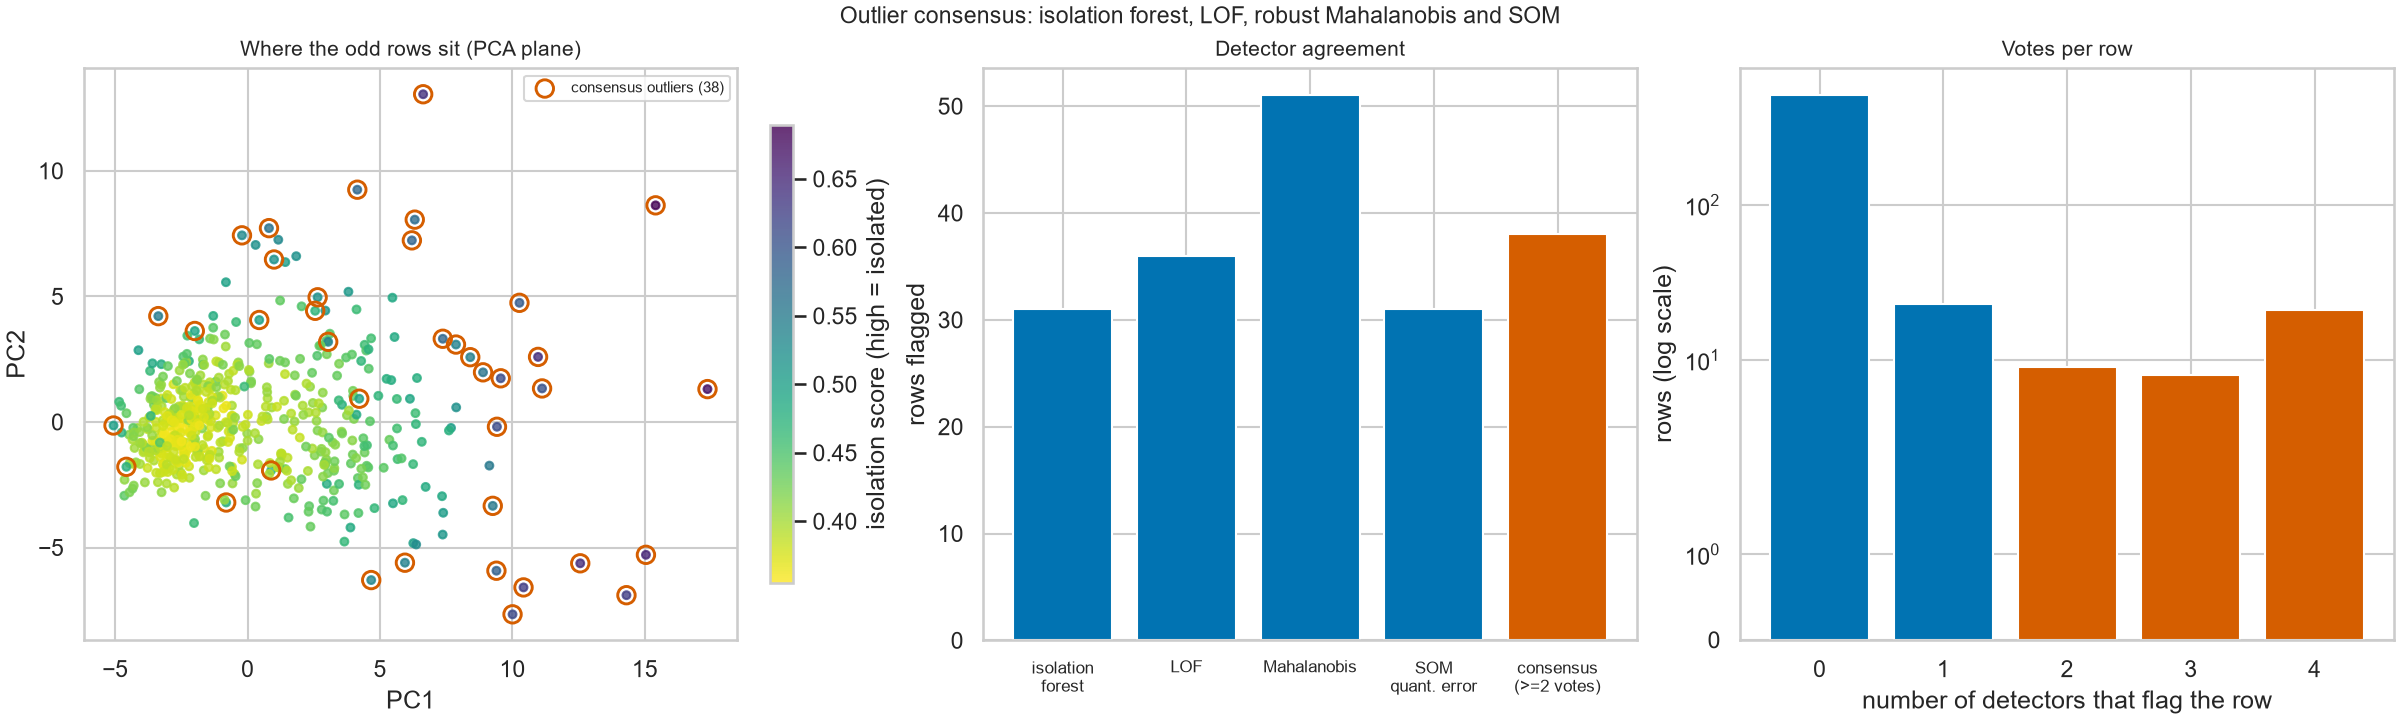
\includegraphics[width=\textwidth]{figures/outlier_consensus.png}\caption{Outlier consensus on the same data. Left: PCA plane coloured by isolation score; rings are consensus outliers. Centre: how many rows each detector flags. Right: number of rows by votes.}\label{fig:cons}\end{figure*}
\begin{figure*}[t]\centering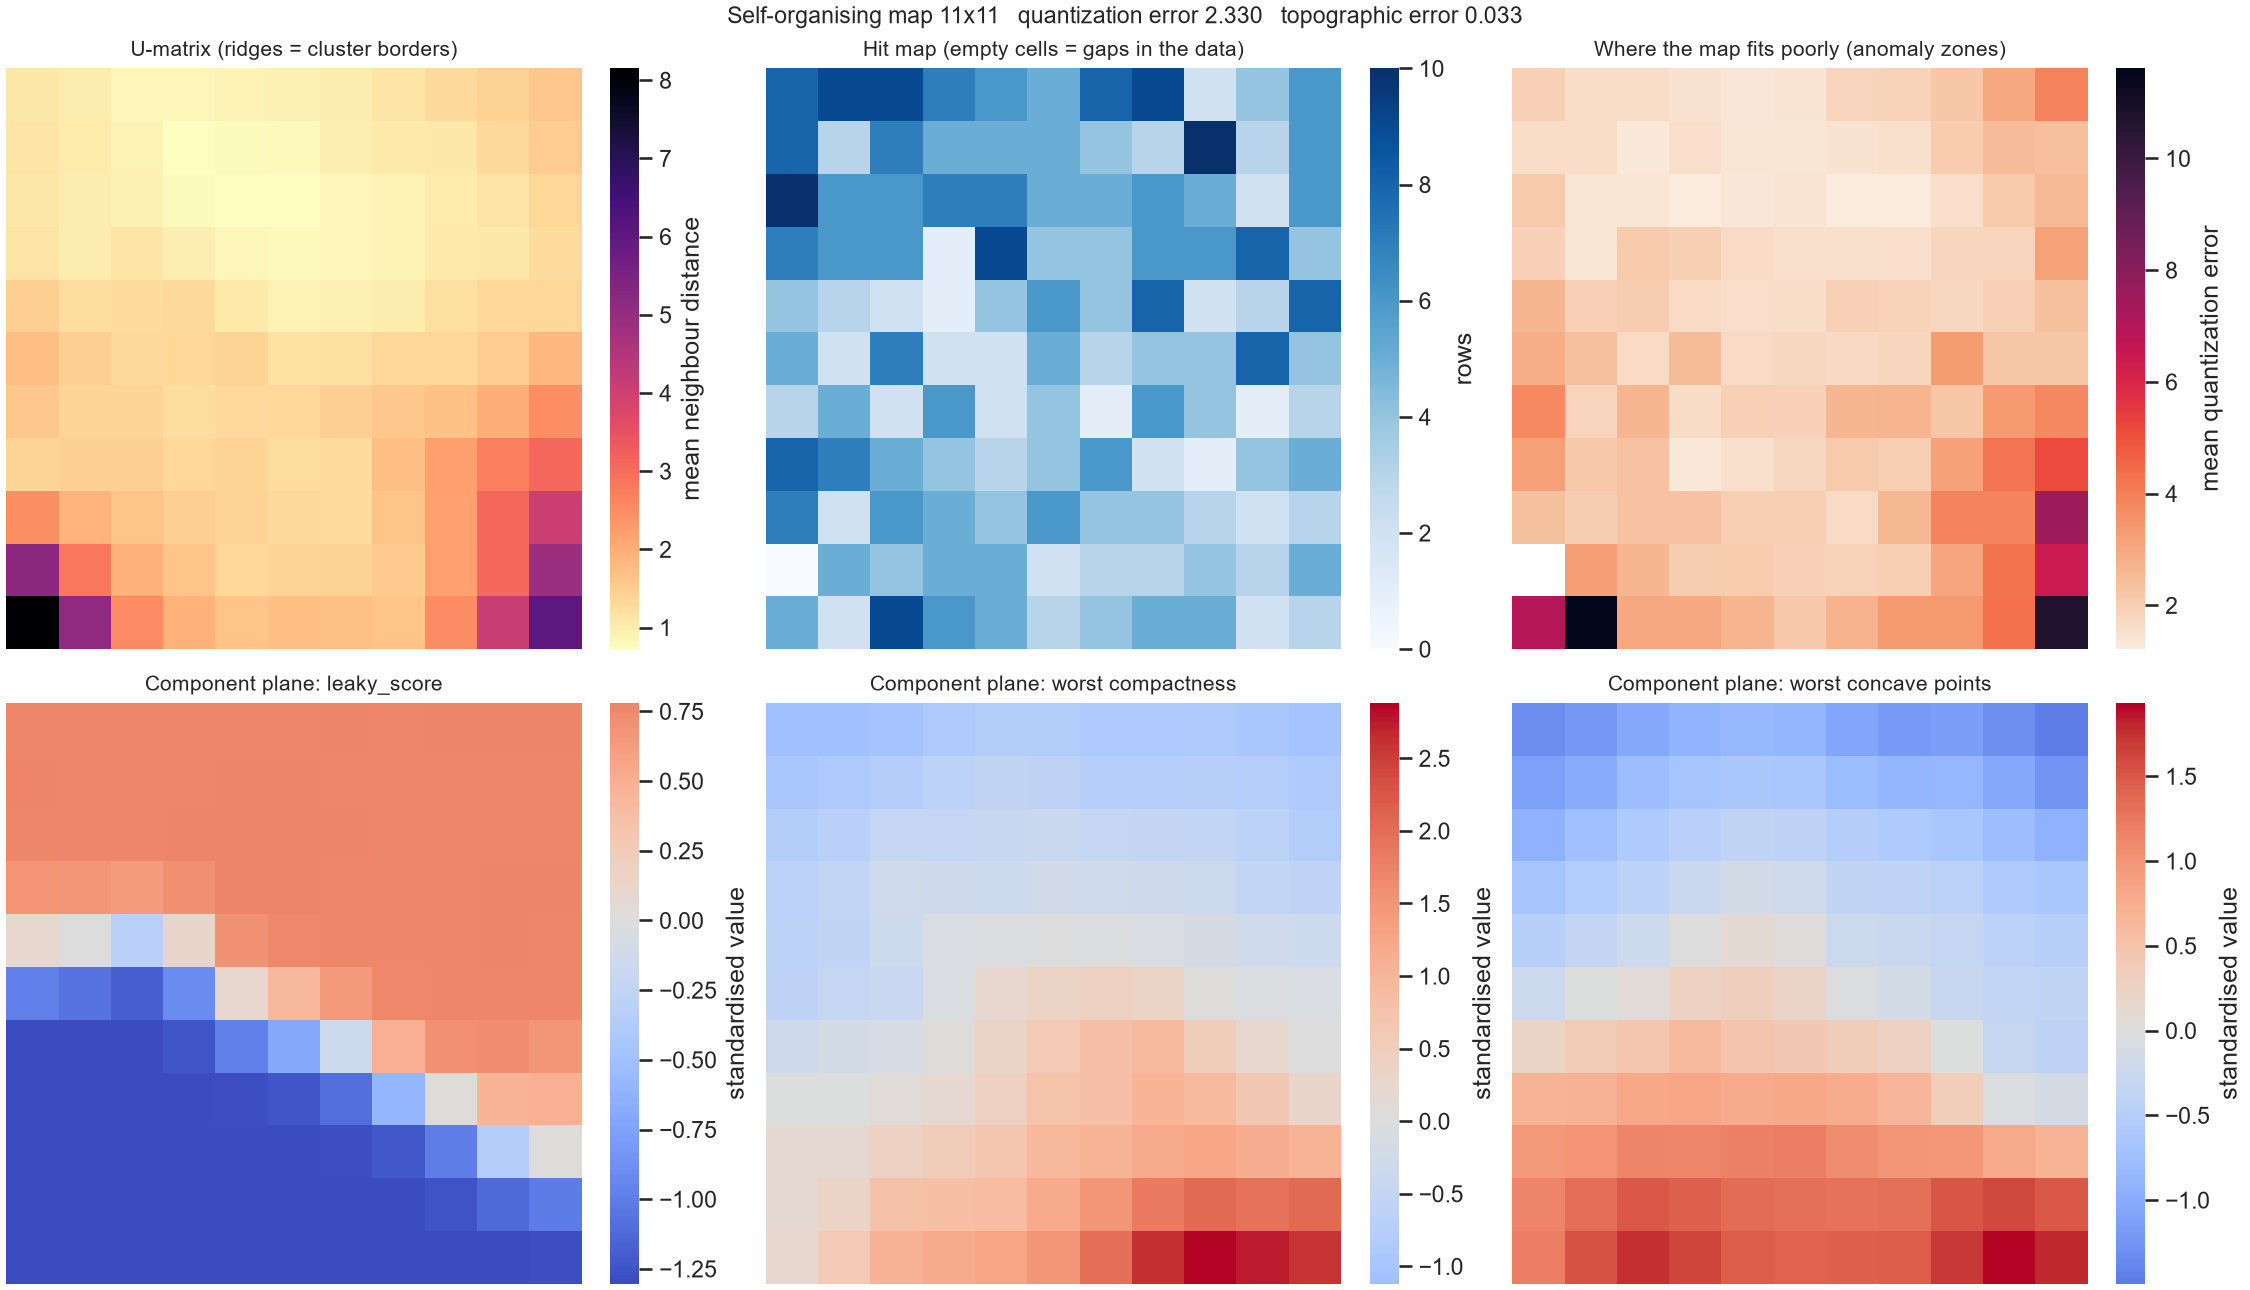
\includegraphics[width=0.9\textwidth]{figures/som.png}\caption{The self-organising map on the same data. Ridges in the U-matrix and the high quantization-error cells in the bottom corners mark the planted extreme rows. The component plane of the planted \code{leaky\_score} column splits the map into two diagonal regions, i.e.\ that single column organises the whole map by class, a visual sign of leakage; the other planes show the two directions along which tumour shape features vary.}\label{fig:som}\end{figure*}
\subsection{Design principles}
(i) Pair a density with its cumulative curve, because histograms hide tails and ECDFs hide modes. (ii) Use log axes for quantities that span orders of magnitude (VIF) and symlog for counts that include zero. (iii) Never encode a quantity that is undefined as zero: units with no hits are blank in the per-unit error map. (iv) Draw the null next to the observation (permutation histogram). (v) Prefer small multiples with shared scales for component planes. (vi) Colour is never the only encoding of a flagged row (rings are used).

\section{Experiments}\label{sec:exp}
All numbers are produced by \code{docs/latex/experiments/data\_intelligence\_experiment.py} and stored in \code{data\_intelligence-results.json}.
\subsection{Planted-outlier benchmark}
Each scenario has $475$ inliers and $25$ planted outliers ($5\%$), $p=6$, $10$ seeds. \emph{Global}: inliers from a correlated Gaussian ($\rho=0.6$), outliers shifted by $5$ standard deviations in every coordinate. \emph{Correlation-breaking}: inliers with $\rho=0.8$, outliers with the same marginals but independent coordinates. \emph{Local density}: a tight cluster ($\sigma=0.3$) and a diffuse one ($\sigma=3$ at $8$); outliers a short distance from the tight cluster, well inside the diffuse cluster's spread. \emph{Between clusters}: three tight clusters at $-6,0,6$ in every coordinate; outliers in the gap near $-3$. Detectors score all rows; we report the area under the ROC curve (AUROC) of the raw score and precision among the top $25$ scores. The ensemble score is the mean normalised rank.
\begin{table*}[t]\caption{AUROC (mean $\pm$ SD over 10 seeds) / precision at 25.}\label{tab:bench}\centering\scriptsize
\begin{tabular}{@{}lccccc@{}}\toprule
Scenario & Isolation forest & LOF & Mahalanobis & SOM quant.\ error & Ensemble rank \\\midrule
Global & $1.000\pm.000$ / 1.00 & $1.000\pm.000$ / 1.00 & $1.000\pm.000$ / 1.00 & $1.000\pm.000$ / 1.00 & $1.000\pm.000$ / 1.00 \\
Correlation-breaking & $.809\pm.031$ / .12 & $.945\pm.019$ / .66 & $.930\pm.024$ / .64 & $.906\pm.029$ / .53 & $.918\pm.024$ / .52 \\
Local density & $.638\pm.040$ / .00 & $\mathbf{.999}\pm.001$ / .96 & $.518\pm.004$ / .00 & $.525\pm.003$ / .00 & $.737\pm.015$ / .00 \\
Between clusters & $\mathbf{.947}\pm.020$ / .32 & $.270\pm.014$ / .00 & $.080\pm.017$ / .00 & $.216\pm.038$ / .00 & $.362\pm.023$ / .00 \\\bottomrule
\end{tabular}\end{table*}
\textbf{Reading the table.} All detectors find gross global outliers. Correlation-breaking outliers are best found by LOF and the Mahalanobis distance, which see the dependence structure, and worst by the isolation forest, whose axis-parallel splits cannot see a broken correlation whose marginals are normal. Local-density outliers are invisible to every global method (AUROC close to $0.5$) and are found almost perfectly by LOF. Between-cluster outliers are the reverse: the three global-in-spirit detectors are \emph{below} $0.5$, because the gap points sit closer to the global centre than the cluster members do (Mahalanobis, AUROC $0.08$), and the SOM absorbs them because units interpolate across the gap (its U-matrix would show a ridge, but its quantization error is small). Only the isolation forest, which isolates points in sparse regions regardless of the centre, is above chance.

\textbf{Consequence for the consensus.} The two-vote rule and the mean-rank ensemble are sensible when outliers are global, but they \emph{dilute} a specialised detector: in the local-density scenario the ensemble precision is zero although LOF is nearly perfect. This is why the report exposes the per-detector counts and \code{single\_detector\_only}, and why we recommend using the ensemble to order the inspection list while reading the individual detector figures to understand \emph{why} a row is listed. No claim is made that the ensemble is superior; the benchmark shows that it is not.

\subsection{Real tables}
\begin{table}[t]\caption{\code{autonomous} mode on bundled datasets (single run; seconds include all stages).}\label{tab:real}\centering\scriptsize
\begin{tabular}{@{}lrrrrrr@{}}\toprule
Dataset & Rows & Cols & Score & Consensus & QE & TE \\\midrule
Breast cancer & 569 & 31 & 66.4 & 34 & 2.39 & .026 \\
Wine & 178 & 14 & 95.5 & 7 & 1.59 & .028 \\
Diabetes & 442 & 11 & 95.5 & 2 & 1.47 & .050 \\\bottomrule
\end{tabular}\end{table}
Wall time was $3.2$\,s for Breast Cancer and about $1$\,s for the other two on a laptop CPU. The Breast Cancer score is lower because its numeric block is strongly collinear (area, radius and perimeter) and contains many heavy-tailed columns; all three targets are declared strongly explained. These tables show feasibility and plausible behaviour, not accuracy of the outlier flags, since the real datasets have no ground-truth outliers.

\subsection{Threats to validity}
The benchmark is synthetic Gaussian and uses fixed detector hyper-parameters; different $k$, $\psi$, grid size or thresholds change the numbers. The cut-offs ($3.5$ robust $z$, $\mathrm{LOF}>1.5$, $\chi^2_{0.999}$) are conventional, not tuned. Sampling at $2000$ rows means flagged row positions refer to the sample. The leakage screen and the feature search are exploratory; a flagged feature may be legitimate. $B=20$ permutations limits the resolution of the explainability p-value.

\section{Analysis toolkit}\label{sec:toolkit}
The engine also ships a toolkit for the questions an analyst asks \emph{after} the first look. Every function returns a dictionary with plain-language findings; all measured numbers below come from \code{docs/latex/experiments/toolkit\_experiment.py} (\code{toolkit-results.json}).
\subsection{Power analysis: predictive, explanatory and statistical}
Let $\hat y_{-i}$ be out-of-fold predictions and $\mathrm{skill}$ be $R^2$ (regression) or chance-adjusted balanced accuracy $(\mathrm{BA}-1/K)/(1-1/K)$. \emph{Predictive power} is $S_{\mathrm{pred}}=\mathrm{skill}(y,\hat y_{-i})$ for ridge and KNN. \emph{Explanatory power} is in-sample: $R^2=1-\mathrm{SSE}/\mathrm{SST}$, $\bar R^2=1-(1-R^2)\frac{n-1}{n-p-1}$, with $F=\frac{R^2/p}{(1-R^2)/(n-p-1)}\sim F_{p,\,n-p-1}$, a per-feature association strength ($r^2$, $\eta^2$ or Cram\'er's $V^2$) with Benjamini--Hochberg adjusted $p$-values~\cite{bh1995}, and for regression the partial $\Delta R^2_j=R^2-R^2_{(-j)}$. The gap $S_{\mathrm{expl}}-S_{\mathrm{pred}}$ measures optimism. \emph{Statistical power} is that of the $F$ test at Cohen's $f^2=R^2/(1-R^2)$~\cite{cohen1988}: $\mathrm{power}=\Pr\!\big(F'_{p,n-p-1}(\lambda)>F_{1-\alpha}\big)$ with non-centrality $\lambda=f^2 n$. The report gives the minimum detectable $f^2$ at power $0.8$ and the $n$ needed for $f^2\in\{0.02,0.15,0.35\}$.
\begin{table}[t]\caption{Power analysis in three regimes ($\alpha=0.05$, power $0.8$).}\label{tab:power}\centering\scriptsize
\begin{tabular}{@{}lrrrl@{}}\toprule
Regime & Ridge CV & KNN CV & In-sample & Verdict \\\midrule
Signal, $n=500,p=5$ & .956 & .849 & .957 & consistent \\
Pure noise & $-.021$ & $-.125$ & .007 & weak on both \\
$n=60,p=30$, noise target & $-1.317$ & $-.308$ & .421 & explains, not predicts \\\bottomrule
\end{tabular}\end{table}
At $n=500$ the minimum detectable $f^2$ is $0.026$ and a medium effect needs $n\ge 92$; at $n=60,p=30$ the minimum detectable $f^2$ is $0.356$, i.e.\ only a very large effect can be established. The linear $F$ approximation is used for classification as well.
\subsection{Comparison, hypothesis tests and A/B testing}
For two groups the engine reports Welch's $t$, the Mann--Whitney $U$ test and Hedges-corrected Cohen's $d=\frac{\bar x_1-\bar x_2}{s_p}\big(1-\frac{3}{4(n_1+n_2)-9}\big)$; for $k\ge3$ groups ANOVA or Kruskal--Wallis with $\eta^2=\mathrm{SSB}/\mathrm{SST}$ and Holm-corrected pairwise Welch tests~\cite{holm1979}. The parametric or rank test is selected by Shapiro--Wilk on each group. For a binary outcome in an A/B test the pooled two-proportion statistic is $z=\frac{\hat p_B-\hat p_A}{\sqrt{\hat p(1-\hat p)(1/n_A+1/n_B)}}$, with a Wald interval for $\hat p_B-\hat p_A$, Fisher's exact test when an expected count is below $5$, and the smallest detectable lift $\delta_{\min}=(z_{1-\alpha/2}+z_{\mathrm{power}})\sqrt{2p(1-p)/n}$. A chi-square test on the arm sizes raises a sample-ratio-mismatch warning. In $200$ simulated null experiments ($1000$ per arm, $10\%$ conversion) the false-positive rate was $0.055$; the power to detect $10\%\to14\%$ was $0.795$.
\subsection{Root-cause search}
Given a bad-outcome indicator $b_i$ with base rate $p_0$, each single condition and each pair of conditions on distinct columns (levels, or terciles of numeric columns) with support $m\ge\max(20,0.02n)$ is scored by lift $=\hat p_S/p_0$ and the one-sided binomial test $\Pr(\mathrm{Bin}(m,p_0)\ge k_S)$, adjusted by Benjamini--Hochberg over all evaluated segments and ranked by excess bad rows $k_S-p_0m$. Numeric features also get a Mann--Whitney AUC between bad and good rows. The result is associational. With a planted segment (\code{region == s} and age above $60$) in $20$ simulated tables the planted segment ranked first $20/20$ times.
\subsection{Time series}
Trend uses the Mann--Kendall statistic $S=\sum_{i<j}\mathrm{sgn}(x_j-x_i)$ with tie-corrected variance and the Sen slope $\mathrm{med}\{(x_j-x_i)/(j-i)\}$~\cite{mann1945,sen1968}. Seasonality is the periodogram peak of the detrended series tested with Fisher's $g=\max_k I_k/\sum_k I_k$ and $p\approx m(1-g)^{m-1}$; the series is decomposed as $x=T+S+R$ with a centred moving-average trend and seasonal strength $F_S=\max(0,1-\mathrm{Var}(R)/\mathrm{Var}(S+R))$. Stationarity combines ADF and KPSS; residual autocorrelation uses Ljung--Box; a level shift is located at $\arg\max_k|\sum_{i\le k}(x_i-\bar x)|$ (CUSUM) with a permutation $p$-value that ignores autocorrelation. On a planted series ($n=365$, slope $0.03$, period $7$, shift $+3$ at $220$) it found period $7$, seasonal strength $0.934$, trend $p<10^{-80}$ and a change point at index $217$; the Sen slope was $0.041$, inflated by the level shift, which shows why the change point should be handled before reading the slope.
\subsection{Iterative, distribution-aware feature construction}
Candidates come from each column's empirical distribution: $\log(1+x)$ if skew $>1$ and $x\ge0$, signed log if $|\mathrm{skew}|>1$, rank-Gauss $\Phi^{-1}\!\big(\frac{\mathrm{rank}+0.5}{n+1}\big)$ if the excess kurtosis exceeds $5$ in magnitude, a density-valley indicator $\mathbb 1[x>t]$ with $t$ the minimum of a Gaussian KDE between the $10$th and $90$th percentiles when it is below $0.6$ of the lower neighbouring mode, and the product, difference, sum and sign-safe ratio of the $6$ columns most correlated with $y$. In each round every candidate $c$ is \emph{screened} with one cross-validated ridge fit, then the top $6$ are \emph{confirmed} over $R=5$ fresh fold assignments with paired gains $g_r=\mathrm{skill}_r(X\cup c)-\mathrm{skill}_r(X)$; it is accepted only if $\bar g-s_g>\tau$ ($\tau=0.002$). The accepted feature joins the pool so later rounds can build on it up to depth $2$. A quarter of the rows is excluded from the search; $\Delta_{\mathrm{hold}}$ is the skill gain on those rows. Constructions are target-free; only selection uses $y$. Over $8$ seeds: planted log-ratio target $\Delta_{\mathrm{hold}}=+0.141$ ($\log(1+\mathrm{price})$ and $\log(1+\mathrm{area})$ were accepted, whose difference is the log-ratio); a planted step on a heavy-tailed column $+0.399$ (the gain came from log, rank and product features, not from the valley threshold, which is conservative and rarely fires); pure noise: $2$ of $8$ runs accepted a feature, mean $\Delta_{\mathrm{hold}}=-0.0009$. The stability rule alone is therefore not a guarantee, and the untouched holdout is what exposes selection optimism.
\subsection{Active learning and row selection}
Starting from a stratified seed of $n_0$ labels, a strategy repeatedly queries a batch from the pool. For class posteriors $p_k(x)$: least confidence $1-\max_k p_k$, margin $-(p_{(1)}-p_{(2)})$, entropy $-\sum p_k\log p_k$, committee vote entropy over $B$ bootstrap models, k-center greedy $\arg\max_x\min_{z\in L}\|x-z\|$, density-weighted margin $u(x)\cdot\bar d_{10}(x)^{-1}$, and our \emph{coverage margin} $u(x)\cdot\frac{d_L(x)}{d_L(x)+\mathrm{med}(d_L)}$ with $u=1-(p_{(1)}-p_{(2)})$ and $d_L$ the distance to the labelled set, updated inside the batch so that a batch is both uncertain and spread out. A label-free farthest-first prefix (\code{diversity\_static}) and any external \code{row\_selector(X,n)} (returned indices only) are static curves. Strategies are compared by the area under the learning curve (ALC), averaged over repeats, with the paired difference to random and its standard deviation.
\begin{table}[t]\caption{ALC (higher is better); $1200$ rows, $5$ repeats.}\label{tab:al}\centering\scriptsize
\begin{tabular}{@{}lrrrrr@{}}\toprule
Data / learner & Random & Margin & Cov.\ margin & Div.\ static & Best \\\midrule
Rings / logistic & .708 & .718 & .704 & .716 & .718 (LC) \\
Rings / KNN & .689 & .712 & .712 & .717 & .717 (DS) \\
Rings / LDA & .706 & .709 & .715 & .708 & .716 (Com.) \\
Imbal. / logistic & .685 & .698 & .710 & .720 & .720 (DS) \\
Imbal. / KNN & .261 & .384 & .480 & .478 & .480 (CM) \\
Imbal. / LDA & .680 & .723 & .718 & .771 & .771 (DS) \\\bottomrule
\end{tabular}\end{table}
No strategy wins everywhere. Gains over random are small for well-behaved learners and large for KNN on imbalanced data, where a good selection also rebalances the classes (so a curve can exceed the all-rows ceiling). The coverage margin is competitive but not uniformly best; we do not claim it dominates the standard strategies. \code{evaluate\_row\_subset} scores any externally chosen subset (skill retained relative to all training rows, mean Kolmogorov--Smirnov distance to the training marginals and class-balance total variation), so a proprietary selector can be compared with these baselines without disclosing its internals.
\begin{figure}[t]\centering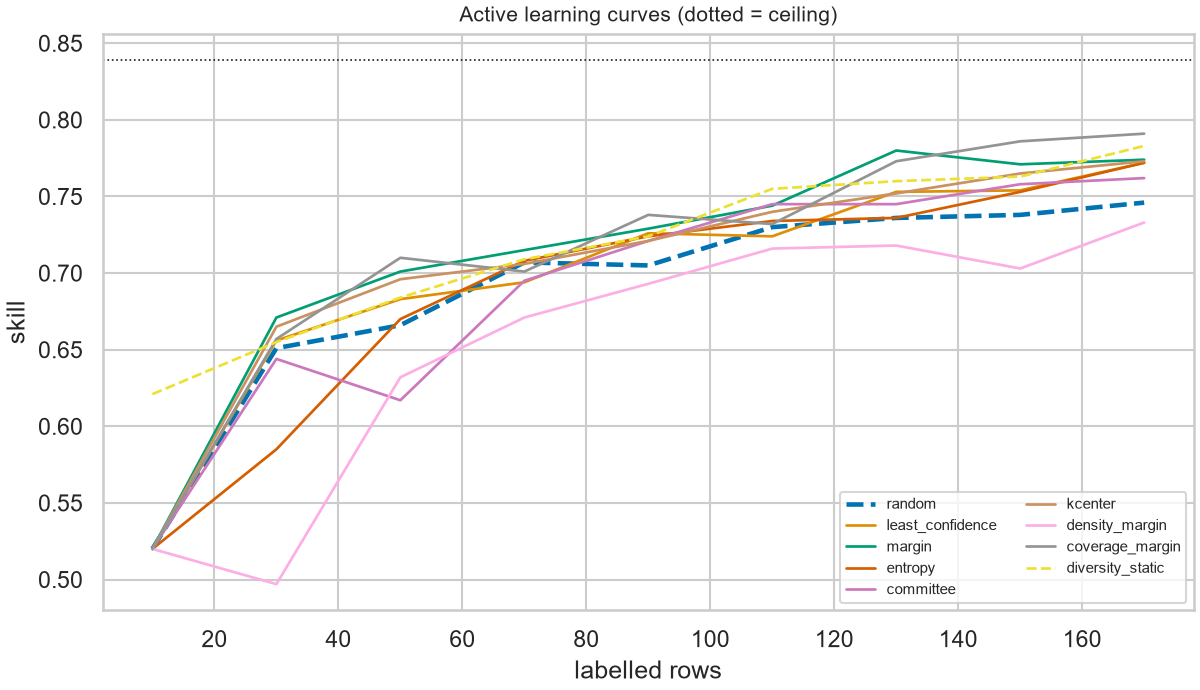
\includegraphics[width=\columnwidth]{figures/toolkit_active_learning.png}\caption{Learning curves for KNN on the rings data (dotted line: skill with all pool rows).}\label{fig:al}\end{figure}
\begin{figure}[t]\centering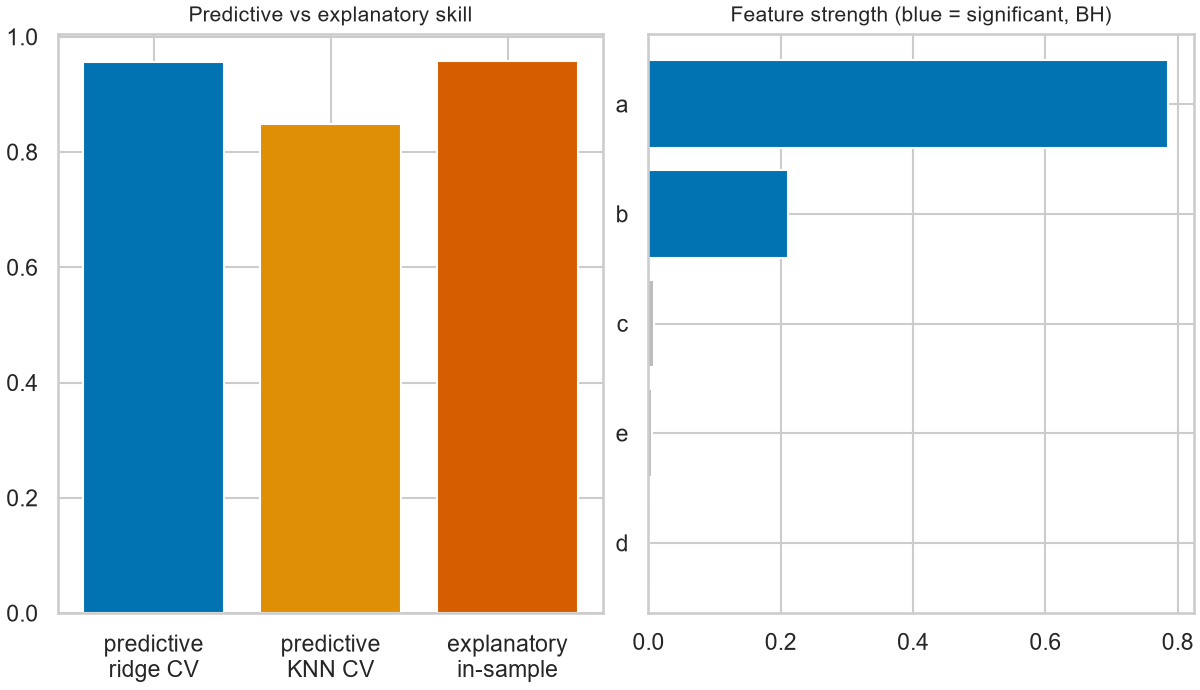
\includegraphics[width=\columnwidth]{figures/toolkit_power.png}\caption{Power analysis, signal regime: predictive vs explanatory skill (left) and per-feature explanatory strength (right).}\label{fig:power}\end{figure}
\subsection{Limits}
The power analysis is a linear approximation; root-cause and group scans are associational; construction is scored with a ridge model; active-learning results are simulations on already labelled data and are not implemented for regression.

\section{Using the engine wisely}
\begin{enumerate}
\item Run \code{DataIntelligence(mode="autonomous")} on the \emph{training} partition and read the dashboard first; a score below about $70$ points to hazards worth fixing before modelling.
\item Act on leakage flags before trusting any selected subset.
\item Prune collinear columns (VIF) if the downstream model is linear or if attributions matter; instance-based or regularised models tolerate more.
\item Read the outlier figures in this order: consensus view (who is odd), SOM (what regions of feature space exist and where the map fits poorly), then the single-detector lists. Decide with domain knowledge whether a row is an error to remove or a case to study; removing hidden-gem rows silently is a modelling decision, not a cleaning step.
\item Persist only when needed: \code{plot\_dir="..."} or \code{export\_dir="..."} (JSON, text and a self-contained HTML with embedded figures). By default nothing is written, which keeps sensitive tables off the disk of a shared machine.
\end{enumerate}

\section{Conclusion}
\code{DataIntelligence} puts target, feature and structure diagnostics in one auditable module whose models are implemented in StatCore and NumPy. The outlier benchmark shows that detectors are complementary rather than interchangeable, so the library reports each of them, a conservative consensus, and the rows that only one detector sees. Future work includes feature-space-aware SOM flags (U-matrix based), kernel or deep detectors, and a tested policy for excluding flagged leakage columns before feature search.

\begin{thebibliography}{9}
\bibitem{liu2008} F. T. Liu, K. M. Ting, and Z.-H. Zhou, ``Isolation forest,'' in \emph{Proc. IEEE Int. Conf. Data Mining (ICDM)}, 2008, pp. 413--422.
\bibitem{breunig2000} M. M. Breunig, H.-P. Kriegel, R. T. Ng, and J. Sander, ``LOF: Identifying density-based local outliers,'' in \emph{Proc. ACM SIGMOD Int. Conf. Management of Data}, 2000, pp. 93--104.
\bibitem{kohonen1982} T. Kohonen, ``Self-organized formation of topologically correct feature maps,'' \emph{Biological Cybernetics}, vol. 43, no. 1, pp. 59--69, 1982.
\bibitem{kohonen2001} T. Kohonen, \emph{Self-Organizing Maps}, 3rd ed. Berlin, Germany: Springer, 2001.
\bibitem{belsley1980} D. A. Belsley, E. Kuh, and R. E. Welsch, \emph{Regression Diagnostics: Identifying Influential Data and Sources of Collinearity}. New York, NY, USA: Wiley, 1980.
\bibitem{rousseeuw1987} P. J. Rousseeuw, ``Silhouettes: A graphical aid to the interpretation and validation of cluster analysis,'' \emph{Journal of Computational and Applied Mathematics}, vol. 20, pp. 53--65, 1987.
\bibitem{software} J. Monchwe \emph{et al.}, ``ReliableML: Reliability-oriented machine learning,'' software repository, \url{https://github.com/Jabualani/ML-Reliabilty}, accessed Oct. 2026.
\bibitem{cohen1988} J. Cohen, \emph{Statistical Power Analysis for the Behavioral Sciences}, 2nd ed. Hillsdale, NJ, USA: Lawrence Erlbaum, 1988.
\bibitem{bh1995} Y. Benjamini and Y. Hochberg, ``Controlling the false discovery rate,'' \emph{J. R. Stat. Soc. B}, vol. 57, no. 1, pp. 289--300, 1995.
\bibitem{holm1979} S. Holm, ``A simple sequentially rejective multiple test procedure,'' \emph{Scand. J. Statist.}, vol. 6, no. 2, pp. 65--70, 1979.
\bibitem{mann1945} H. B. Mann, ``Nonparametric tests against trend,'' \emph{Econometrica}, vol. 13, no. 3, pp. 245--259, 1945.
\bibitem{sen1968} P. K. Sen, ``Estimates of the regression coefficient based on Kendall's tau,'' \emph{J. Am. Stat. Assoc.}, vol. 63, pp. 1379--1389, 1968.
\bibitem{settles2009} B. Settles, ``Active learning literature survey,'' Univ. Wisconsin--Madison, Comput. Sci. Tech. Rep. 1648, 2009.
\end{thebibliography}
\end{document}
